\documentclass[a4paper,12pt]{article}

\usepackage[T2A]{fontenc}
\usepackage[utf8]{inputenc}
\usepackage[russian]{babel}

\usepackage{geometry}
\geometry{margin=2.2cm}

\usepackage{hyperref}
\hypersetup{
  colorlinks=true,
  linkcolor=blue,
  urlcolor=blue
}

\usepackage{graphicx}
% build_pdf.bat компилирует из block1/2.4/solution/explanation/_temp,
% поэтому картинки, лежащие в ../charts, должны находиться.
\graphicspath{{../charts/}{charts/}}

\usepackage{float}
\usepackage{amsmath}
\usepackage{booktabs}

% Если microtype вдруг подключается (шаблоном/скриптом/кем-то ещё),
% то отключаем expansion, чтобы не ловить "auto expansion only possible with scalable fonts".
\makeatletter
\@ifpackageloaded{microtype}{\microtypesetup{expansion=false}}{}
\makeatother

\title{Task 2.4 --- Counters: JMH + Scalability}
\author{Данил}
\date{}

\begin{document}
\maketitle
\sloppy

\section{Экспериментальная установка}

Измерения производительности выполнены с помощью JMH в режиме \texttt{Throughput}
(единицы \texttt{ops/ms}). Использовались сценарии:
\begin{itemize}
  \item \texttt{get-only}: benchmark вызывает только \texttt{get()}
  \item \texttt{increment-only}: benchmark вызывает только \texttt{increment()}
\end{itemize}

Сравнивались реализации счётчика:
\begin{itemize}
  \item \texttt{ThreadUnsafeCounter} (без синхронизации)
  \item \texttt{LockedCounter} на \texttt{ReentrantLock} (\texttt{fair=false} и \texttt{fair=true})
  \item \texttt{SplitCounter} (lock splitting) с разной гранулярностью
\end{itemize}

\paragraph{Про «не оптимизировал ли компилятор нагрузку» (DCE).}
JMH старается защищать измерения от выбрасывания «мертвого» кода.
Дополнительно в тестовом наборе (и при построении графиков) используется реальное чтение результата
\texttt{get()}, что делает эффект вычислений наблюдаемым, а значит их нельзя просто выкинуть как ненужные.

\section{Easy}

\subsection{ThreadUnsafeCounter}

Реализация:
\begin{itemize}
  \item \texttt{increment(): data++}
  \item \texttt{get(): return data}
\end{itemize}

\paragraph{Корректность.}
\texttt{ThreadUnsafeCounter} не потокобезопасен: операция \texttt{data++} не атомарна
(чтение $\rightarrow$ увеличение $\rightarrow$ запись). Поэтому при конкурентных инкрементах
часть обновлений может теряться, а \texttt{get()} может наблюдать состояния, которые не соответствуют
«идеальному» последовательному счётчику.

\paragraph{Масштабируемость.}
В \texttt{get-only} обычно масштабируется хорошо, т.к. это просто чтение переменной.
В \texttt{increment-only} throughput может выглядеть высоким, но корректность результата не гарантируется.

\subsection{NoContentionBaseline}

\texttt{NoContentionBaseline} запускает $N$ потоков, где каждый поток увеличивает \textbf{свой} приватный счётчик.
Это baseline без contention: общих данных нет, поэтому при увеличении числа потоков throughput растёт,
пока не исчерпаны аппаратные ресурсы CPU.

\subsection{LockedCounter: ReentrantLock}

\texttt{LockedCounter} использует один общий \texttt{ReentrantLock} для защиты переменной \texttt{data}.
Рассмотрены два режима:
\begin{itemize}
  \item \textbf{unfair} (\texttt{fair=false})
  \item \textbf{fair} (\texttt{fair=true})
\end{itemize}

\paragraph{Масштабируемость.}
Обе реализации масштабируются плохо: все потоки конкурируют за один lock,
поэтому появляется узкое место и throughput быстро выходит на плато.

\paragraph{Oversubscription.}
При числе потоков больше числа CPU рост throughput прекращается и часто появляется деградация:
увеличиваются накладные расходы планировщика и число переключений контекста.

\paragraph{Fair vs Unfair.}
\texttt{fair=true} обычно медленнее: требуется поддерживать справедливую очередь ожидания,
что увеличивает парковки/пробуждения потоков и scheduler overhead.
\texttt{fair=false} чаще позволяет «перехватывать» lock потоку, который уже на CPU,
поэтому может давать больший throughput.

\subsection{Выводы Easy}

\begin{itemize}
  \item Между unsafe и lock-based реализациями есть разрыв по single-thread throughput из-за стоимости lock/unlock.
  \item \texttt{get} масштабируется лучше, чем \texttt{increment} (особенно в lock-based вариантах).
  \item Один общий lock (\texttt{LockedCounter}) почти сразу становится bottleneck.
  \item \texttt{fair=true} обычно снижает throughput из-за дополнительных издержек планировщика.
\end{itemize}

\section{Medium}

\subsection{SplitCounter (lock splitting)}

\texttt{SplitCounter} использует массив «порций» \texttt{portions[]} и массив lock'ов \texttt{locks[]}.
Индекс порции выбирается по идентификатору потока:
\[
  idx = threadId \bmod granularity
\]

\paragraph{increment.}
\texttt{increment()} блокирует ровно один lock (\texttt{locks[idx]}) и увеличивает \texttt{portions[idx]}.

\paragraph{get.}
\texttt{get()} блокирует \textbf{все} locks, суммирует все порции и затем освобождает locks.
Это даёт согласованный снимок: на время \texttt{get} инкременты блокируются.

\subsection{Корректность и тесты}

\paragraph{Почему корректно.}
\begin{itemize}
  \item Каждый инкремент защищён lock'ом соответствующей порции, поэтому обновления не теряются внутри порции.
  \item \texttt{get} удерживает все locks на время суммирования, поэтому результат соответствует согласованному состоянию
  «между» операциями \texttt{increment}.
\end{itemize}

\paragraph{Тесты.}
Добавлены тесты корректности, включая стресс-тесты:
\begin{itemize}
  \item single-thread: точная сумма после многих инкрементов;
  \item стабильность \texttt{get} без инкрементов;
  \item стресс: много потоков, точная сумма после завершения;
  \item стресс: конкурентные \texttt{get} во время инкрементов;
  \item стресс: oversubscription + таймаут против зависаний.
\end{itemize}

\subsection{Масштабируемость и oversubscription}

\paragraph{increment масштабируется лучше.}
За счёт распределения по порциям уменьшается contention: потоки не стоят в одной очереди к одному lock.

\paragraph{get масштабируется хуже.}
\texttt{get} создаёт глобальную точку синхронизации (lock-all), поэтому параллелизм не помогает.
Кроме того, при большой гранулярности стоимость \texttt{get} растёт из-за необходимости захвата множества lock'ов.

\paragraph{Oversubscription.}
При потоков больше CPU throughput перестаёт расти (или падает),
так как увеличиваются переключения контекста. Для \texttt{increment} splitting обычно переносит
oversubscription лучше, чем один lock, но рост всё равно ограничен CPU.

\subsection{Коллизии порций и аналогия}

Можно искусственно увеличить contention, если выбрать маленькую гранулярность
относительно числа потоков: многие потоки будут попадать в одну порцию, и выигрыш от splitting снизится.

Аналогия в однопоточных структурах: \textbf{hash table} с коллизиями (несколько ключей в одном bucket).
Как уменьшить проблему:
\begin{itemize}
  \item увеличить \texttt{granularity} (больше «buckets»);
  \item улучшить распределение потоков по порциям (уменьшить перекос);
  \item использовать динамическое расширение (как делают реальные структуры).
\end{itemize}

\section{Графики производительности}

Ниже приведены графики throughput (ops/ms) в зависимости от числа потоков.
Error bars взяты из \texttt{scoreError} JMH.

\begin{figure}[H]
  \centering
  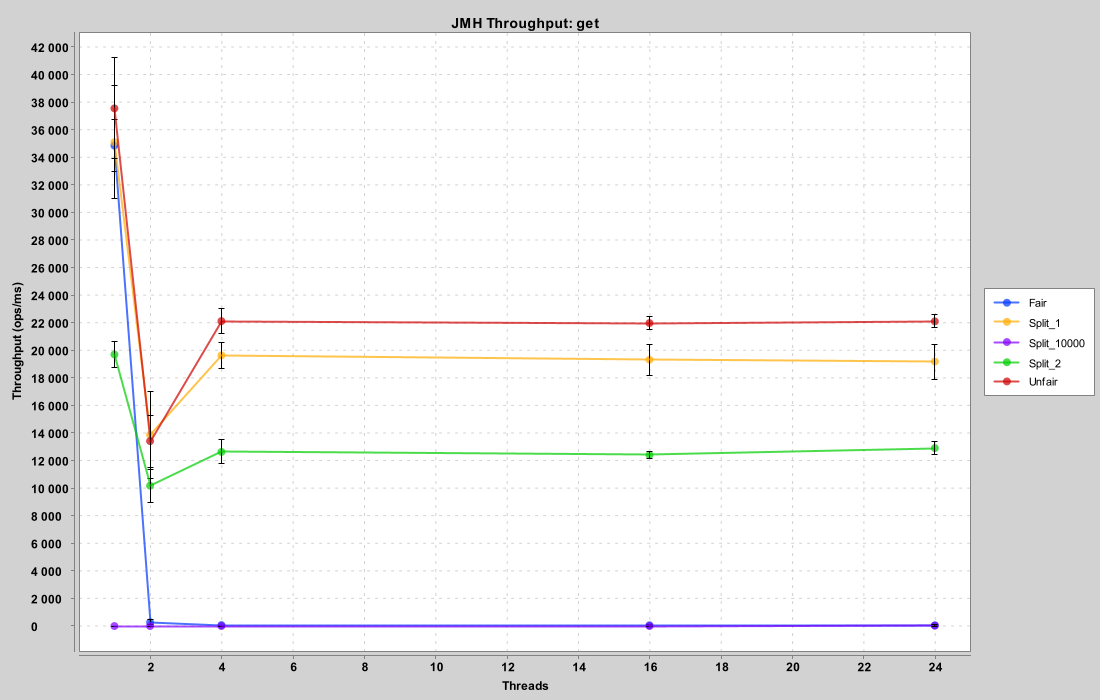
\includegraphics[width=0.95\textwidth]{throughput_get.png}
  \caption{Throughput vs Threads: get-only}
\end{figure}

\begin{figure}[H]
  \centering
  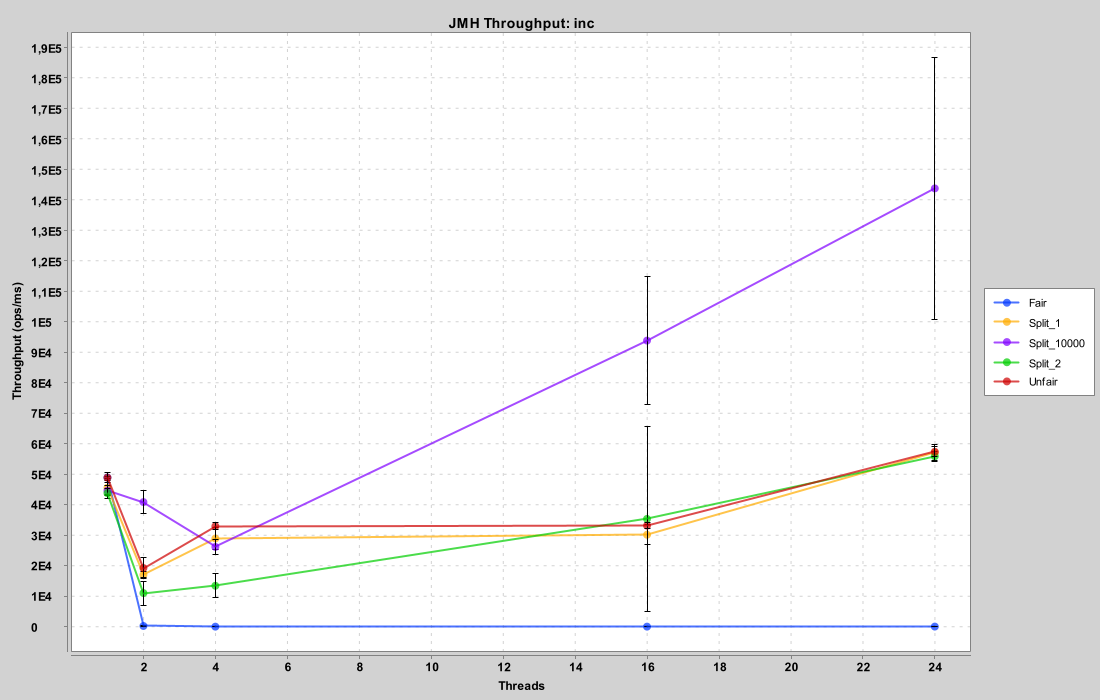
\includegraphics[width=0.95\textwidth]{throughput_inc.png}
  \caption{Throughput vs Threads: increment-only}
\end{figure}

\section{Итоговые выводы}

\begin{itemize}
  \item \texttt{ThreadUnsafeCounter} даёт высокий throughput, но не гарантирует корректность при конкурентных инкрементах.
  \item \texttt{LockedCounter} корректен, но плохо масштабируется из-за contention на одном lock.
  \item \texttt{fair=true} обычно снижает throughput за счёт overhead планировщика и дополнительных переключений контекста.
  \item \texttt{SplitCounter} улучшает масштабируемость \texttt{increment}, но делает \texttt{get} дороже (lock-all).
\end{itemize}

\end{document}